\chapter{Proposed methodology and planning}
\label{chapter:methodology}

The main goal of this work is to implement and demonstrate a real-time object detector in a FPGA-based development board. Taking into account the study performed in chapter \ref{chapter:object_detection}, the YOLOv3 detector presents the best trade-off between accuracy and execution time. The Deep Versat system, introduced in chapter \ref{chapter:cgra}, alongside the techniques for CNN acceleration in FPGAs studied in chapter \ref{chapter:DNN}, will be used to implement the detector.

\section{Infrastructure}
\label{section:infrastructure}

The development board available for this work is the Kintex UltraScale KU040~\cite{fpga}. To receive images in real-time, the cost-effective OV7670 camera module~\cite{camera} was chosen as it can be easily connected to the PMOD modules of the board. This camera operates at maximum 30 fps and has a maximum resolution of 640x480 pixels. Given the interfaces available on the board, the HDMI interface was selected to display the resulting images in a monitor. The proposed infrastructure is represented in Fig.~\ref{fig:infrastructure}. 

\begin{figure}[!htb]
  \centering
  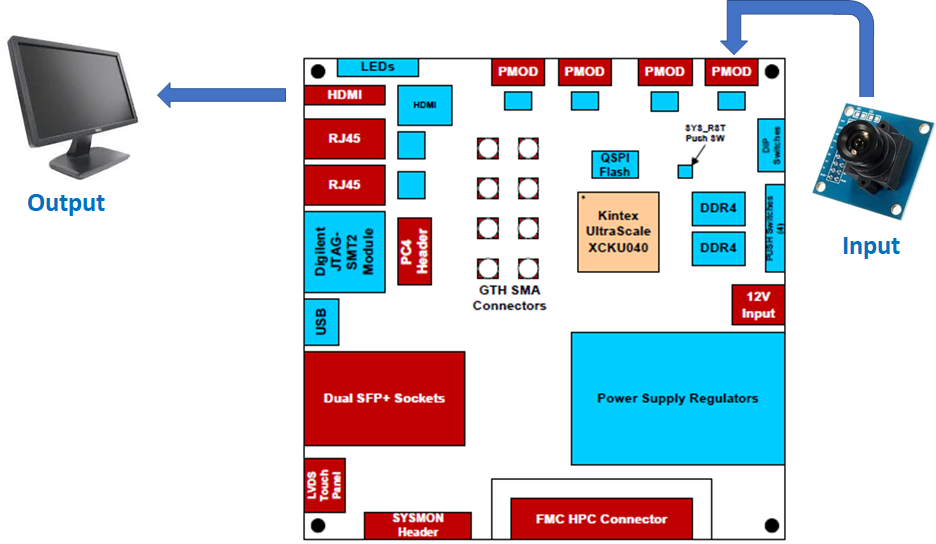
\includegraphics[width=0.85\textwidth]{Figures/fpga_system.png}
  \caption{Composition of the proposed infrastructure (adapted from~\cite{fpga}).}
  \label{fig:infrastructure}
\end{figure}

\subsection{OV7670 camera module}

The pinout of the camera is represented in Table~\ref{tab:ov7670}. The camera has two different communication protocols: one for its configuration and another for data acquisition. The pins SDIOD and SDIOC are used for configuring the camera using a specific protocol similar to I2C. Possible configurations include the data output format (e.g., RGB565, YCbCr 4:2:2), the frame resolution (e.g., 640x480, 320x240) and the frame rate. For this work, the camera will be configured in the RGB565 format with a resolution of 640x480 and a frame rate of 30 fps.

\begin{table}[!htb]
    \footnotesize
    \centering
    \caption{Parameters of the dual-port memories.}
    \label{tab:ov7670}
    \begin{tabular}{|c|c|c|c|c|}
    \hline
    Type & Pin & Description & Pin &  Description \\ \hline
    Supply & VDD & Power supply & GND & Ground \\ \hline
    Input/Output & SDIOD & Control bus data & \multicolumn{2}{c|}{} \\ \hline
    \multirow{2}{*}{Input} & SDIOC & Control bus clock & XCLK & System clock \\ \cline{2-5}
    & RESET & Reset (active low) & PWDN & Power down (active high) \\ \hline
    \multirow{2}{*}{Output} & VSYNC & Vertical synchronization & HREF & Horizontal synchronization \\ \cline{2-5}
    & PCLK & Pixel clock & D0-D7 & Pixel parallel output \\ \hline
    \end{tabular}
\end{table}

Changing the configuration corresponds to updating the value of a specific register in the camera module. When idle, both SDIOC and SDIOD are at logical one. The data transmission starts by driving the SDIOC pin at logical zero. A logical one during data transmission indicates that one bit was sent. The SDIOD pin can only change while SDIOC is at logical zero. After transmitting the address of the register and the value to be updated, the pins are driven at logical one, indicating the end of the transmission.

The pixel data is transmitted in parallel (8 bits). First, a frequency between 10 and 48 MHz must be supplied to the XCLK pin~\cite{camera}. As shown in Fig.~\ref{fig:data_acquisition}, the 640 pixels that form one row must be captured while HREF is at logical one and the 480 rows are acquired while VSYNC is at logical zero. The data must be sampled at the rising edge of the PCLK signal. For the RGB565 format, two clock cycles are needed to collect each pixel. The reset and power down signals are kept at logical zero and logical one.

\begin{figure}[!htb]
  \centering
  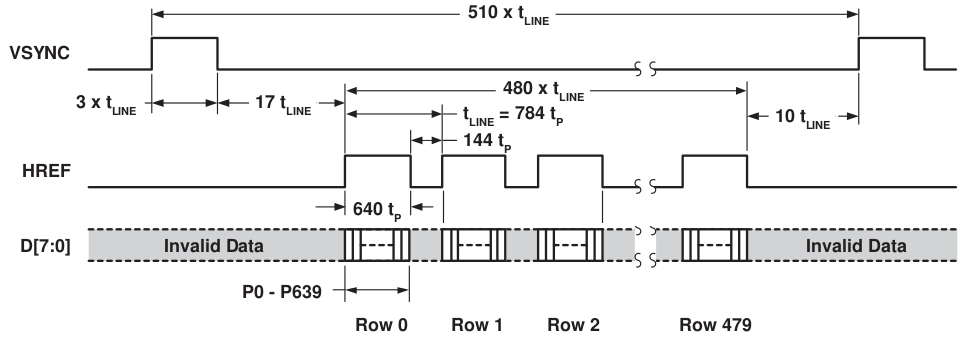
\includegraphics[width=0.85\textwidth]{Figures/camera_data_acquisition.png}
  \caption{Protocol for the camera data acquisition~\cite{camera}.}
  \label{fig:data_acquisition}
\end{figure}

\vspace{-0.2cm}
\subsection{HDMI module}

The board has an ADV7511 HDMI transmitter~\cite{hdmi} to drive the interface. Although the ADV7511 module accepts 36 bits per pixel, the board is only connected to 16 pixels (from bit 8 to bit 23)~\cite{fpga}. As a consequence, the format of the data must be YCbCr 4:2:2. This implies a color space conversion from the RGB format of the camera to the YCbCr format of the HDMI interface~\cite{color_conversion}:

\begin{equation}
    %\syslineskipcoeff{1}
    \normalsize 
    \systeme*{ Y = 16 + \frac{65.738}{256} \times R + \frac{129.057}{256} \times G + \frac{25.064}{256} \times B, Cb = 128 - \frac{37.945}{256} \times R - \frac{74.494}{256} \times G + \frac{112.439}{256} \times B, Cr = 128 + \frac{112.439}{256} \times R - \frac{94.194}{256} \times G - \frac{18.285}{256} \times B}
\end{equation}
\vspace{+0.2cm}

The video streams have active video periods and blanking periods, as represented in Fig.~\ref{fig:active_video} . Only the active video is shown on the display. When transmitting video, the signals HSYNC (horizontal synchronization), VSYNC (vertical synchronization) and DE (data enable) must be generated.

\begin{figure}[!htb]
  \centering
  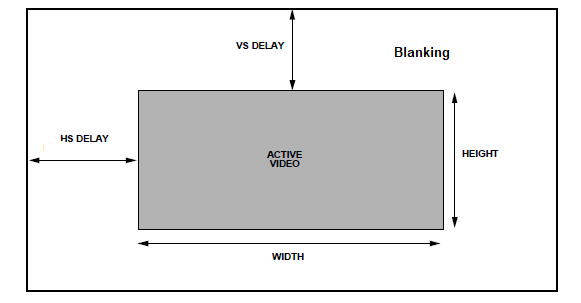
\includegraphics[width=0.7\textwidth]{Figures/active_video.png}
  \caption{Active video (adapted from~\cite{camera}.)}
  \label{fig:active_video}
\end{figure}

A logic one DE indicates an active pixel (i.e., the visual part of the video signal) and a logic zero DE indicates the blanking period of the video signal. The generation of the DE is represented in Fig.~\ref{fig:hdmi_signals}. The range of values for the synchronization signals depends on the resolution being used. For configurations such as the data format, the I2C protocol is used.

\begin{figure}[!htb]
  \centering
  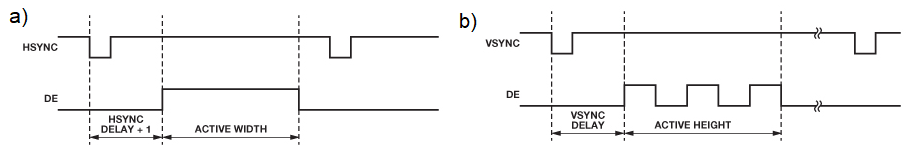
\includegraphics[width=\textwidth]{Figures/hdmi_signals.png}
  \caption{a) Horizontal and b) vertical DE generation (adapted from~\cite{camera}).}
  \label{fig:hdmi_signals}
\end{figure}

The camera and HDMI modules will be developed in Verilog. These modules will be integrated as peripherals in the Deep Versat system as represented in Fig.~\ref{fig:final_system}. 

\begin{figure}[!htb]
  \centering
  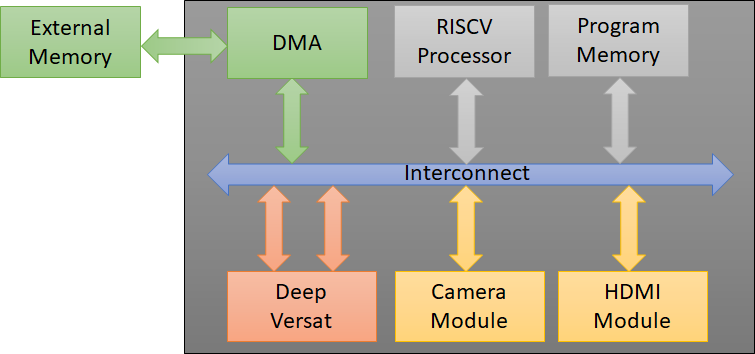
\includegraphics[width=0.6\textwidth]{Figures/final_system.png}
  \caption{Integration of the modules in the Deep Versat system.}
  \label{fig:final_system}
\end{figure}

\section{Planning}
\label{section:planning}

This thesis work is planned for a period of nine months, as shown in the Gantt Chart presented in Fig. \ref{fig:planning}. The first task will consist in implementing a software-only version of the YOLOv3 detector in the RISC-V processor to be used as baseline. As this processor currently does not support floating point operations, the application will need to be already converted to fixed point arithmetic by applying a pre-defined quantization. The detector will initially be based on the YOLOv3-Tiny network.

For the second task, the convolutional layers will be accelerated using the Deep Versat architecture. Following the approach in previous works, a design space exploration will be conducted in order to find the best parameters for the loop optimization techniques, namely the unroll and tiling factors.

Furthermore, a study will be conducted in order to measure the impact of implementing the other layers and other routines of the detector (e.g., image resize, non-maximum suppression) in the RISC-V processor. If after accelerating the convolutional layers, the bottleneck of the application resides on any of these routines, then hardware-based alternatives will have to be considered. For instance, the logistic operation performed by the yolo layers can be approximated by using pre-defined values stored in LUTs. 

The following two tasks will focus on the deployment of the camera and HDMI modules for the infrastructure proposed in this chapter. Finally, the system will be fully integrated and tested. The thesis will be written throughout the implementation of the work. 

\begin{figure}[!htb]
  \centering
  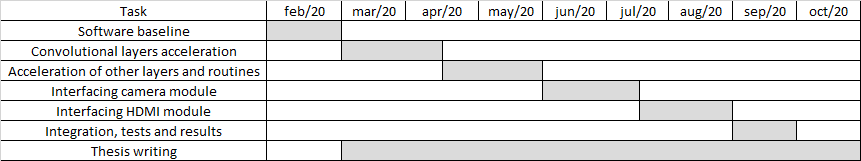
\includegraphics[width=\textwidth]{Figures/gantt.png}
  \caption{Planning of the thesis.}
  \label{fig:planning}
\end{figure}

\subsubsection{Final remarks}

The expected results with the development of this work include the infrastructure for receiving images from the OV7670 camera in real-time and displaying the resulting images from the YOLOv3 detector in an HDMI monitor. For the YOLOv3-Tiny network, the expected frame rate should be near the maximum frame rate of the camera (i.e., 30 fps).  